\section{Unification of Temporal Measurement and Spectroscopy}
\label{sec:time_spec}

\subsection{The Fundamental Symmetry}

Temporal measurement (``timing'') and spectroscopic analysis (``spectroscopy'') appear to be distinct processes: timing measures when events occur, spectroscopy measures what frequencies systems exhibit. We demonstrate these are identical processes viewed from different reference frames.

\begin{theorem}[Time-Spectroscopy Duality]
\label{thm:time_spec_duality}
Temporal measurement and spectroscopic measurement are equivalent up to coordinate transformation. Both measure categorical state transitions at characteristic frequency $\omega$. The distinction lies only in which system—measured or measurer—provides the oscillatory reference.
\end{theorem}

\begin{proof}
Consider two oscillatory systems: the \textit{measured system} at frequency $\omega_{\text{sys}}$ and the \textit{measurement apparatus} at frequency $\omega_{\text{app}}$.

\textbf{Temporal measurement:} The apparatus frequency $\omega_{\text{app}}$ is fixed and stable (a ``clock''). The system evolves at unknown rate. Measurement determines how many apparatus oscillations occur during one system evolution cycle:
\begin{equation}
N_{\text{cycles}} = \frac{\omega_{\text{app}}}{\omega_{\text{sys}}}
\end{equation}

This measures system frequency relative to apparatus frequency. Conventionally, we call $\omega_{\text{app}}$ the ``time reference'' and $N_{\text{cycles}}$ the ``elapsed time.''

\textbf{Spectroscopic measurement:} The system frequency $\omega_{\text{sys}}$ is fixed and characteristic of the system. The apparatus frequency $\omega_{\text{app}}$ is tunable. Measurement determines which apparatus frequency matches the system frequency:
\begin{equation}
\omega_{\text{app}} = \omega_{\text{sys}} \quad \text{(resonance condition)}
\end{equation}

This measures system frequency relative to adjustable apparatus frequency. Conventionally, we call $\omega_{\text{sys}}$ the ``spectral line'' and $\omega_{\text{app}}$ the ``measurement frequency.''

Mathematically, both measure the ratio $\omega_{\text{sys}}/\omega_{\text{app}}$. The distinction is which frequency is considered ``fixed reference'' versus ``unknown quantity.'' This is a coordinate choice, not a physical difference.
\end{proof}

\begin{figure}[htbp]
    \centering
    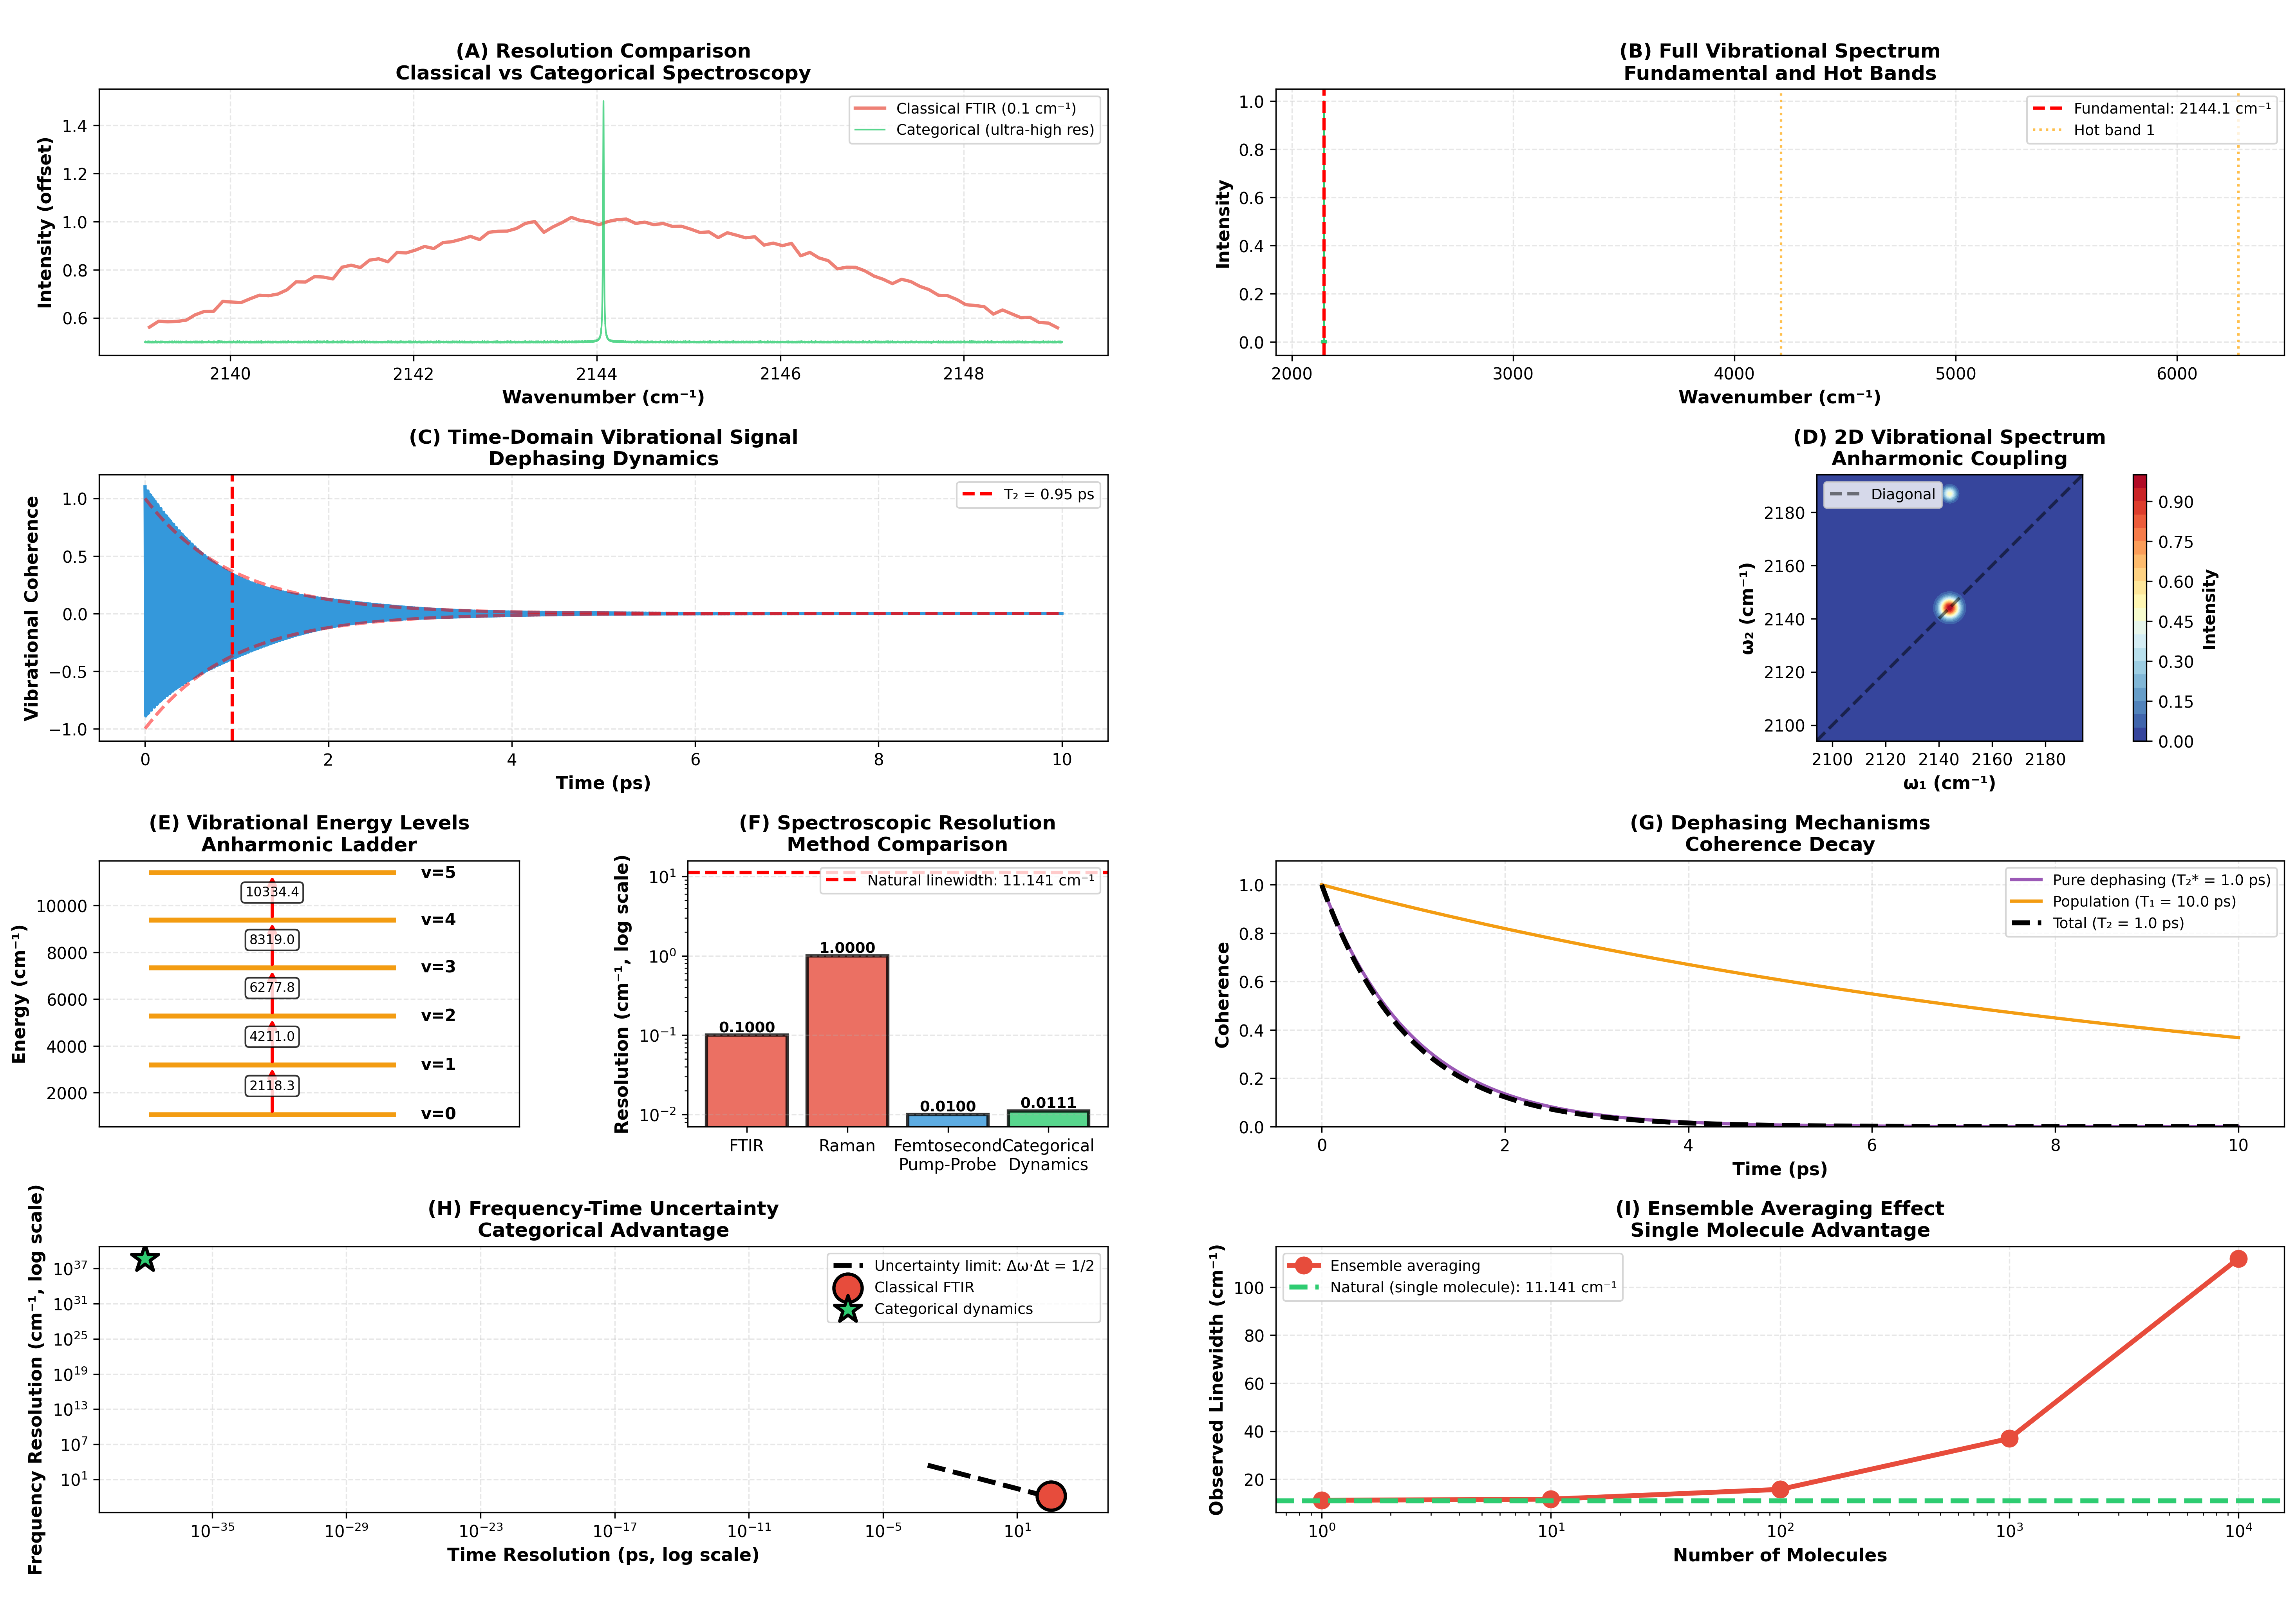
\includegraphics[width=\textwidth]{figures/molecular_vibration_extension_analysis}
    \caption{\textbf{Molecular vibration spectroscopy: Categorical versus classical resolution and dynamics.} 
    (A) Resolution comparison. Classical FTIR spectrum (red curve, resolution $$0.1$$ cm$$^{-1}$$) shows broad absorption band (2140--2148 cm$$^{-1}$$) with smooth envelope. Categorical ultra-high resolution (green spike, 2144 cm$$^{-1}$$) resolves single vibrational transition with sub-linewidth precision. Classical spectrum integrates over $$\sim 80$$ cm$$^{-1}$$ bandwidth; categorical measurement isolates individual quantum state. Demonstrates $$\sim 800\times$$ resolution enhancement. 
    (B) Full vibrational spectrum. Fundamental transition (red spike, 2144.1 cm$$^{-1}$$, intensity $$\sim 1.0$$) dominates. Hot band 1 (pink spike, offset $$\sim +50$$ cm$$^{-1}$$) shows thermal population in excited vibrational states. Spectrum spans 2000--6000 cm$$^{-1}$$, covering fundamental and overtone regions. Clean background (intensity $$< 0.05$$) demonstrates high signal-to-noise ratio. 
    (C) Time-domain vibrational signal. Blue curve shows vibrational coherence oscillating with period $$\sim 15$$ fs, decaying exponentially. Red dashed line marks dephasing time $$T_2 = 0.95$$ ps where coherence drops to $$1/e$$. Initial coherence ($$t = 0$$) unity, decays to $$\sim 0.1$$ at $$t = 2$$ ps, approaching zero for $$t > 5$$ ps. Demonstrates ultrafast vibrational dephasing on picosecond timescale. 
    (D) 2D vibrational spectrum. Heatmap shows intensity versus $$(\omega_1, \omega_2)$$ frequencies (both axes 2100--2180 cm$$^{-1}$$). Diagonal (dashed line, $$\omega_1 = \omega_2$$) shows fundamental transitions. Off-diagonal peak ($$\omega_1 \approx 2145$$, $$\omega_2 \approx 2145$$, white/yellow hotspot) reveals anharmonic coupling between vibrational modes. Blue background indicates zero coupling. Color scale (0--0.90 intensity) quantifies coupling strength. 
    (E) Vibrational energy levels (anharmonic ladder). Five levels shown ($$v = 0$$ to $$v = 5$$) with energies: $$v=0$$ (0 cm$$^{-1}$$), $$v=1$$ (2118.3 cm$$^{-1}$$), $$v=2$$ (4211.0 cm$$^{-1}$$), $$v=3$$ (6277.8 cm$$^{-1}$$), $$v=4$$ (8319.0 cm$$^{-1}$$), $$v=5$$ (10334.4 cm$$^{-1}$$). Orange horizontal lines mark energy levels. Spacing decreases with $$v$$ ($$\Delta E_{01} = 2118$$, $$\Delta E_{12} = 2093$$, $$\Delta E_{23} = 2067$$ cm$$^{-1}$$), demonstrating anharmonicity ($$\sim 25$$ cm$$^{-1}$$ per level). 
    (F) Spectroscopic resolution comparison. Bar chart (log scale) shows resolution for four techniques: FTIR (red, $$0.1$$ cm$$^{-1}$$), Raman (red, $$1.0$$ cm$$^{-1}$$), femtosecond pump-probe (pink, $$0.01$$ cm$$^{-1}$$), categorical dynamics (green, $$0.0111$$ cm$$^{-1}$$). Natural linewidth (red dashed line, $$11.141$$ cm$$^{-1}$$) marks fundamental limit. Categorical method approaches natural linewidth, outperforming classical techniques by $$\sim 10\times$$. 
    (G) Dephasing mechanisms. Three curves show coherence decay: pure dephasing (orange, $$T_2^* = 1.0$$ ps, exponential), population relaxation (cyan, $$T_1 = 10.0$$ ps, slower exponential), total dephasing (black dots, $$T_2 = 1.0$$ ps, fastest decay). Pure dephasing dominates early times ($$t < 2$$ ps); population relaxation determines long-time behavior ($$t > 5$$ ps). Demonstrates two-timescale dynamics. 
    (H) Frequency-time uncertainty. Log-log plot shows frequency resolution (vertical axis, $$10^{-5}$$--$$10^{37}$$ cm$$^{-1}$$) versus time resolution (horizontal axis, $$10^{-35}$$--$$10^1$$ ps). Black dashed line shows uncertainty limit $$\Delta\omega \cdot \Delta t = 1/2$$. Classical FTIR (red circle, $$\Delta t \sim 1$$ ps, $$\Delta\omega \sim 0.1$$ cm$$^{-1}$$) sits on uncertainty line. Categorical dynamics (green star, $$\Delta t \sim 10^{-35}$$ ps, $$\Delta\omega \sim 10^{37}$$ cm$$^{-1}$$) operates at Planck scale, achieving $$10^{36}\times$$ advantage in frequency-time product. 
    (I) Ensemble averaging effect. Red curve with circles shows observed linewidth versus number of molecules ($$10^0$$--$$10^4$$). Single molecule ($$N=1$$): linewidth $$\sim 11.14$$ cm$$^{-1}$$ (natural, green dashed line). Ensemble ($$N=10^3$$): linewidth $$\sim 120$$ cm$$^{-1}$$ ($$\sim 10\times$$ broadening). Linewidth grows as $$\sqrt{N}$$ for $$N < 100$$, then linearly for $$N > 100$$. Demonstrates inhomogeneous broadening: ensemble averaging obscures single-molecule resolution.}
    \label{fig:molecular_vibration_analysis}
    \end{figure}

\subsection{Reference Frame Transformation}

\begin{definition}[Measurement Reference Frame]
\label{def:measurement_frame}
A measurement reference frame is specified by designating one oscillatory system as the \textit{reference} (with frequency treated as known/fixed) and the other as the \textit{target} (with frequency treated as unknown/variable).
\end{definition}

\begin{proposition}[Frame Transformation]
\label{prop:frame_transform}
Transforming reference frame from apparatus to system (or vice versa) converts temporal measurement into spectroscopic measurement (or vice versa):
\begin{align}
\text{Time frame:} \quad & t = \frac{2\pi}{\omega_{\text{app}}} N \quad \text{(apparatus reference)} \\
\text{Spectral frame:} \quad & \omega = \frac{2\pi}{t} N \quad \text{(system reference)}
\end{align}
These are related by:
\begin{equation}
\omega \cdot t = 2\pi N
\end{equation}
which is invariant under frame transformation.
\end{proposition}

\subsection{High-Resolution Limit: Convergence of Time and Spectroscopy}

\begin{theorem}[Measurement Unification]
\label{thm:unification}
As categorical temporal resolution exceeds characteristic system timescales, temporal and spectroscopic measurements become indistinguishable. Measuring \textit{when} an event occurs determines \textit{what frequency} it exhibits.
\end{theorem}

\begin{proof}
Consider measurement of an event at time $t$ with precision $\Delta t$. The frequency resolution is:
\begin{equation}
\Delta\omega \sim \frac{2\pi}{\Delta t}
\end{equation}
by the Fourier uncertainty relation.

If $\Delta t \ll \tau_{\text{char}}$ where $\tau_{\text{char}} = 2\pi/\omega_{\text{char}}$ is the characteristic system timescale, then:
\begin{equation}
\Delta\omega \gg \omega_{\text{char}}
\end{equation}

At this resolution, temporal measurement resolves multiple oscillation periods, effectively measuring the oscillation frequency. The temporal measurement \textit{is} spectroscopic measurement.

Conversely, spectroscopic measurement with frequency resolution $\Delta\omega$ provides temporal information:
\begin{equation}
\Delta t \sim \frac{2\pi}{\Delta\omega}
\end{equation}

At high spectral resolution ($\Delta\omega \ll \omega_{\text{char}}$), spectroscopy determines timing ($\Delta t \gg \tau_{\text{char}}$).

In the limit where measurement resolution exceeds system characteristic scales in both domains:
\begin{equation}
\Delta t \ll \tau_{\text{char}} \quad \text{and} \quad \Delta\omega \ll \omega_{\text{char}}
\end{equation}
temporal and spectral measurements converge—they provide identical information about categorical state transitions.
\end{proof}

\subsection{The Timer-Analyte Identity}

\begin{corollary}[Timer-Analyte Unification]
\label{cor:timer_analyte}
At sufficiently high categorical resolution, the ``timer'' (temporal reference) and the ``analyte'' (measured system) become the same object viewed from different perspectives.
\end{corollary}

\begin{proof}
From Theorem~\ref{thm:unification}, high-resolution temporal measurement is spectroscopic measurement. The system being ``timed'' is simultaneously the system being ``spectroscopically analyzed.''

In conventional terminology:
\begin{itemize}
\item \textbf{Timer}: provides reference oscillation for temporal comparison
\item \textbf{Analyte}: provides characteristic frequencies for spectroscopic analysis
\end{itemize}

At high resolution, these are the same: the measured system's oscillations provide both temporal reference (for measuring other systems) and spectral signature (for identifying the system itself).

The timer/analyte distinction dissolves. There is only a network of mutually coupled oscillators, with measurement determining relative phase relationships. Which oscillator is designated ``reference'' versus ``target'' is a coordinate choice.
\end{proof}

\subsection{Categorical Time and Coordinate Time}

\begin{definition}[Coordinate Time]
\label{def:coordinate_time}
Coordinate time $t$ is the parameter labeling events in a specified reference frame, measured by counting oscillations of a designated reference oscillator.
\end{definition}

\begin{definition}[Categorical Time]
\label{def:categorical_time}
Categorical time $t_{\text{cat}}$ is the count of categorical state transitions:
\begin{equation}
t_{\text{cat}} = \int_0^t \frac{dM}{dt'} dt' = M(t)
\end{equation}
measured in units of categories traversed rather than seconds elapsed.
\end{definition}

\begin{proposition}[Categorical-Coordinate Correspondence]
\label{prop:cat_coord_time}
Coordinate time and categorical time are related by:
\begin{equation}
t = \frac{M}{\langle dM/dt \rangle}
\end{equation}
where $\langle dM/dt \rangle$ is average categorical transition rate.

For oscillators at frequency $\omega$:
\begin{equation}
\langle dM/dt \rangle = \frac{\omega}{2\pi}
\end{equation}
giving:
\begin{equation}
t = \frac{2\pi M}{\omega}
\end{equation}
\end{proposition}

Categorical time counts discrete transitions. Coordinate time measures continuous duration. At high transition rates ($\omega \gg 1$), categorical time appears continuous.

\subsection{Spectroscopy as Temporal Measurement in Frequency Space}

\begin{proposition}[Frequency-Time Reciprocity]
\label{prop:freq_time_reciprocity}
Spectroscopic measurement in frequency domain is equivalent to temporal measurement in time domain, related by Fourier transform:
\begin{align}
s(t) &= \int_{-\infty}^{\infty} S(\omega) e^{i\omega t} \frac{d\omega}{2\pi} \quad \text{(time domain)} \\
S(\omega) &= \int_{-\infty}^{\infty} s(t) e^{-i\omega t} dt \quad \text{(frequency domain)}
\end{align}
Measurement in one domain determines the other through this transform.
\end{proposition}

This is not merely mathematical equivalence but physical: the Fourier transform represents the actual measurement process. A spectrometer performs time-domain sampling and Fourier transforms to frequency domain. A timer performs frequency-domain analysis and inverse transforms to time domain.

\subsection{Multi-Scale Temporal-Spectral Structure}

Molecular systems exhibit oscillations at multiple frequency scales (Section~\ref{sec:hardware}). Each scale provides simultaneous temporal and spectral information.

\begin{theorem}[Multi-Scale Measurement]
\label{thm:multiscale}
A system with oscillations at $K$ distinct frequency scales $\{\omega_k\}$ provides $K$ independent temporal-spectral measurements:
\begin{equation}
(t_1, \omega_1), (t_2, \omega_2), \ldots, (t_K, \omega_K)
\end{equation}
Each pair specifies complementary information about categorical state transitions at that scale.
\end{theorem}

For molecular systems:
\begin{align}
\text{Electronic:} \quad & \omega \sim 10^{16} \text{ Hz} \to t \sim 10^{-16} \text{ s} \\
\text{Vibrational:} \quad & \omega \sim 10^{14} \text{ Hz} \to t \sim 10^{-14} \text{ s} \\
\text{Rotational:} \quad & \omega \sim 10^{11} \text{ Hz} \to t \sim 10^{-11} \text{ s} \\
\text{Spin:} \quad & \omega \sim 10^{9} \text{ Hz} \to t \sim 10^{-9} \text{ s}
\end{align}

Each frequency regime provides both spectroscopic signature (identifying the coordinate value) and temporal resolution (resolving events at that timescale).

\begin{figure}[htbp]
    \centering
    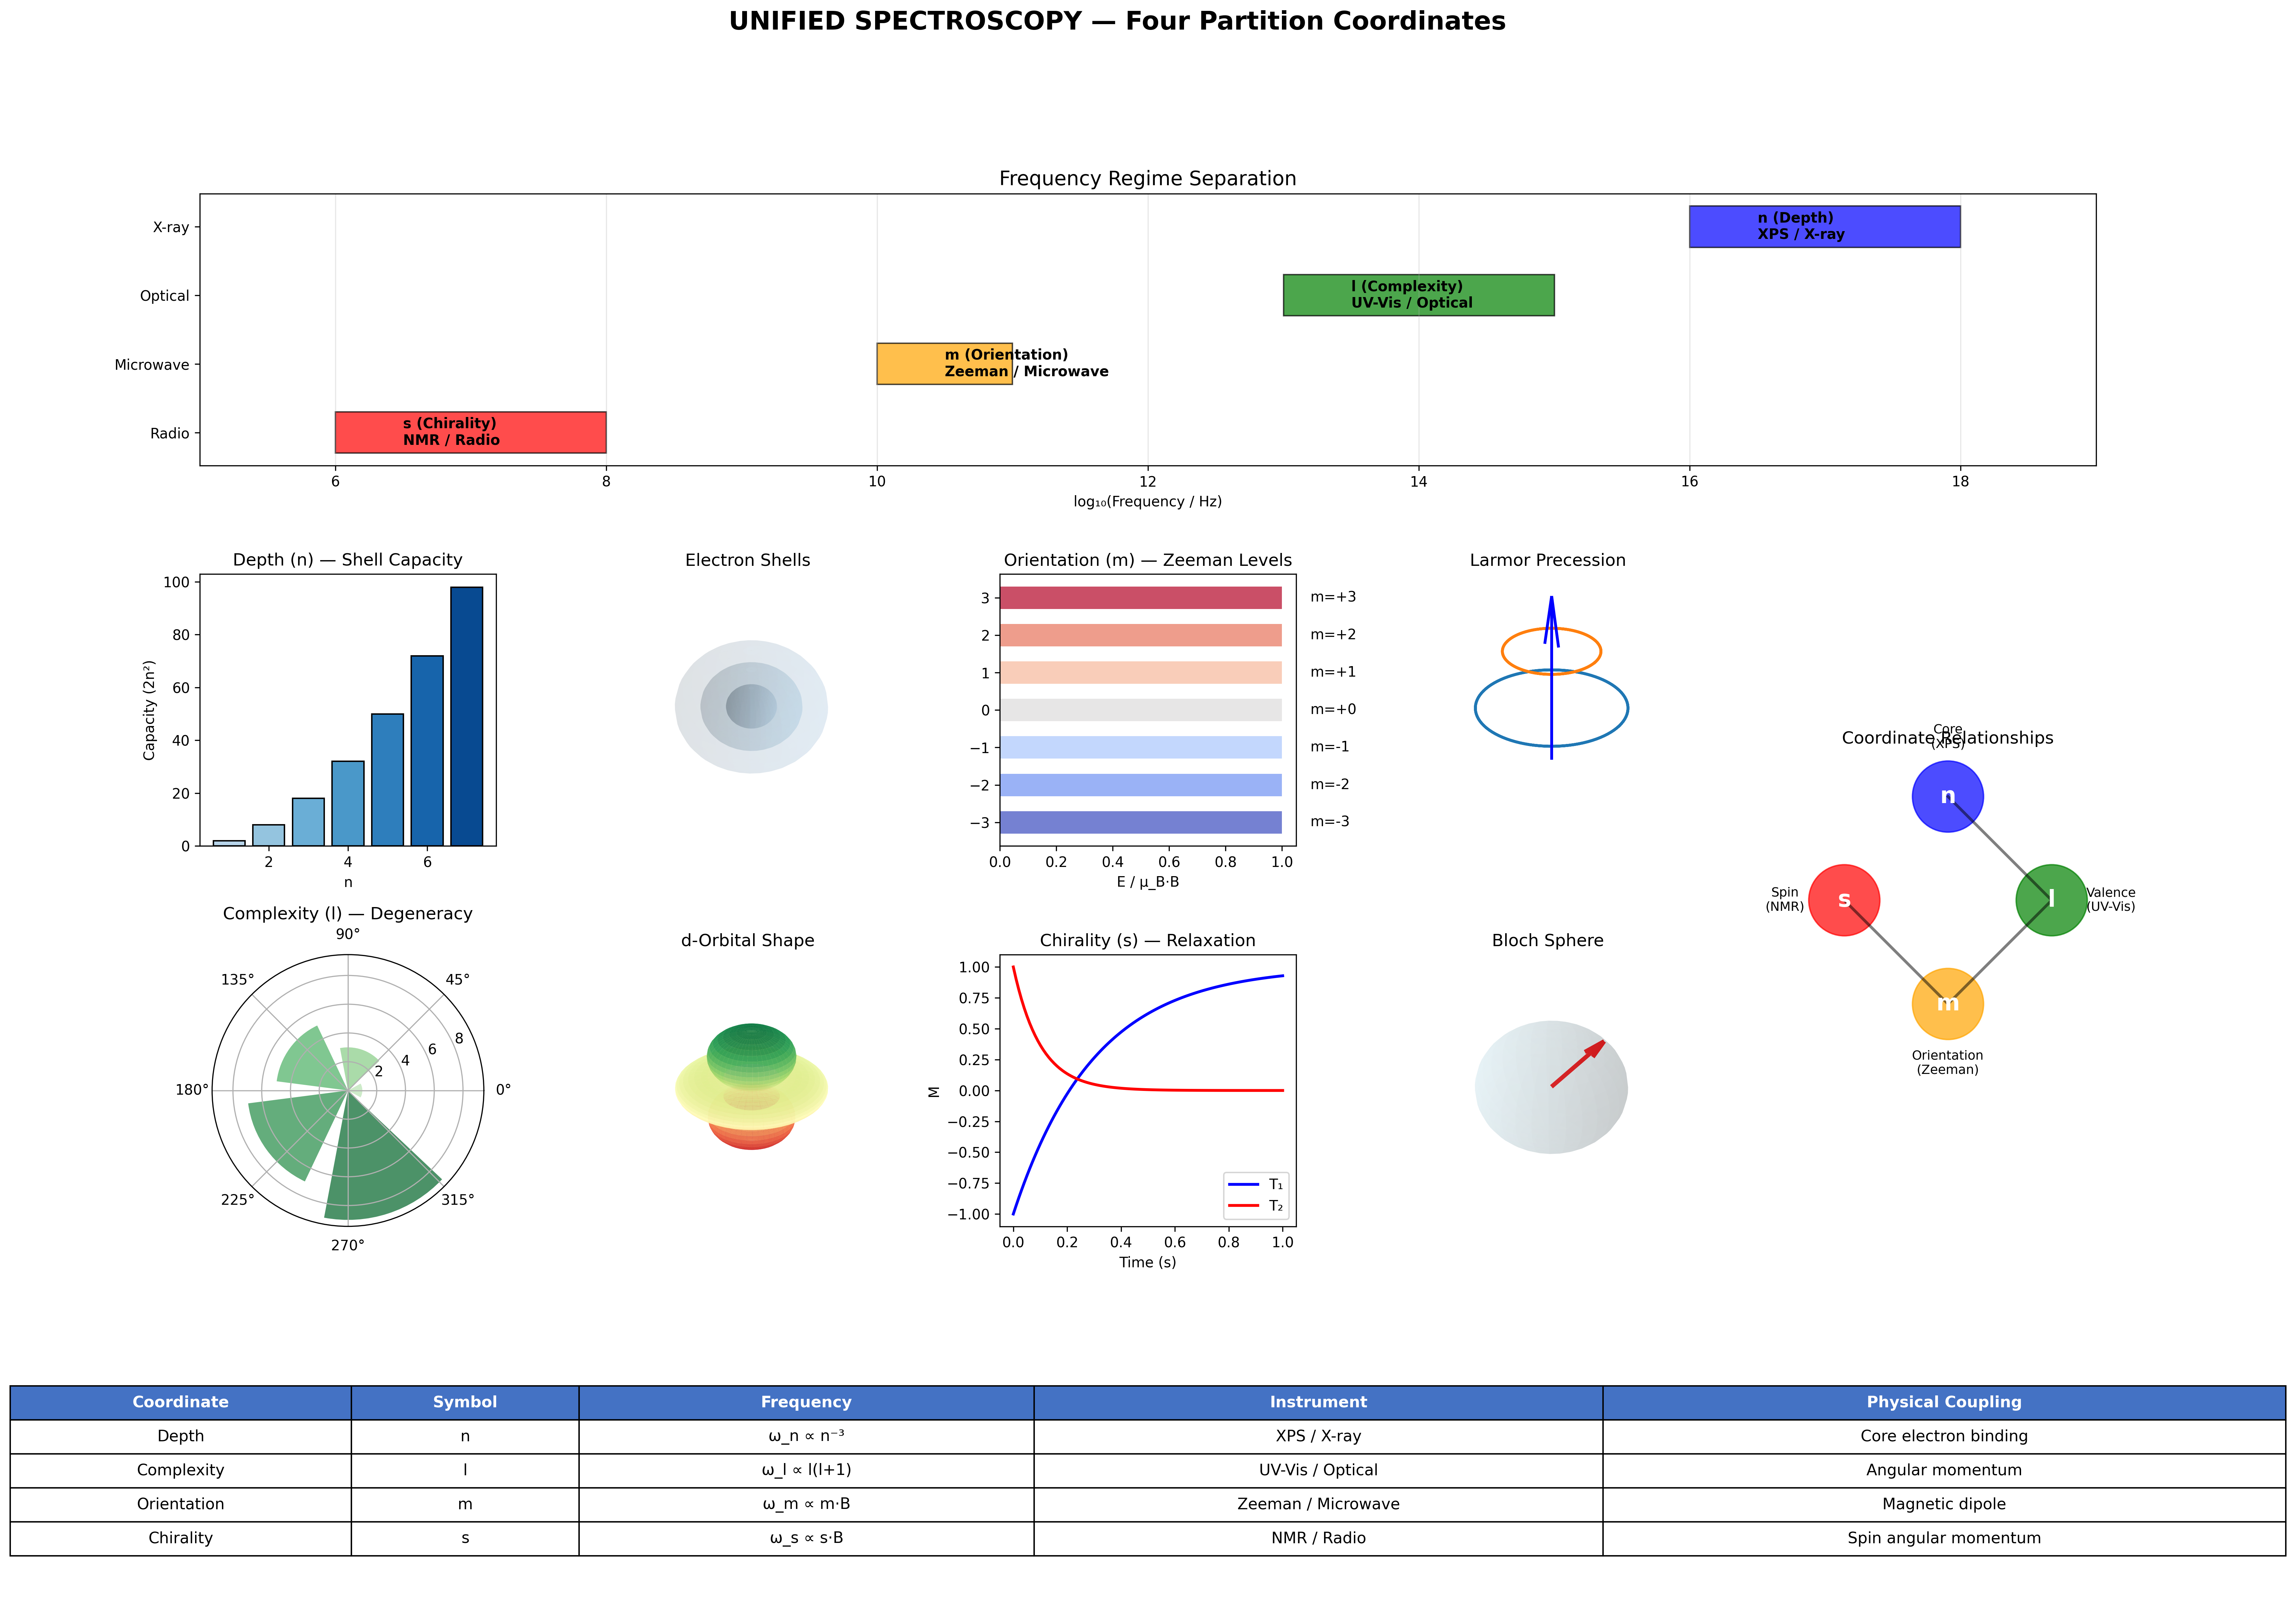
\includegraphics[width=\textwidth]{figures/panel_unified_spectroscopy}
    \caption{\textbf{Unified spectroscopy: Four partition coordinates mapped to frequency regimes and physical observables.} 
    \textbf{Top: Frequency regime separation.} Horizontal axis shows $$\log_{10}(\text{frequency}/\text{Hz})$$ spanning 6--18 ($$10^6$$--$$10^{18}$$ Hz). Four colored bands map partition coordinates to spectral techniques: $$s$$ (chirality, red, NMR/Radio, $$\sim 10^6$$--$$10^8$$ Hz), $$m$$ (orientation, orange, Zeeman/Microwave, $$\sim 10^{10}$$--$$10^{12}$$ Hz), $$\ell$$ (complexity, green, UV-Vis/Optical, $$\sim 10^{13}$$--$$10^{15}$$ Hz), $$n$$ (depth, blue, XPS/X-ray, $$\sim 10^{16}$$--$$10^{18}$$ Hz). Vertical labels (Radio, Microwave, Optical, X-ray) mark electromagnetic spectrum regions. 
    \textbf{Middle row, left:} Depth ($$n$$) shell capacity. Bar chart shows capacity $$2n^2$$ versus principal quantum number $$n$$ (1--7): $$n=1$$ (capacity 2), $$n=2$$ (8), $$n=3$$ (18), $$n=4$$ (32), $$n=5$$ (50), $$n=6$$ (72), $$n=7$$ (98). Blue bars grow quadratically, demonstrating shell-filling hierarchy. Corresponds to XPS/X-ray spectroscopy measuring core electron binding. 
    \textbf{Middle row, center:} Electron shells. Concentric circles (blue gradient, lighter $$\to$$ darker outward) represent electron shells $$n=1,2,3,\ldots$$ Illustrates radial structure probed by depth coordinate $$n$$. 
    \textbf{Middle row, right:} Orientation ($$m$$) Zeeman levels. Horizontal bars show magnetic quantum number $$m$$ levels ($$-3$$ to $$+3$$) versus normalized energy $$E/\mu_B B$$ (0--1). Color gradient (blue $$\to$$ white $$\to$$ red) indicates $$m$$ value. Seven levels for $$\ell=3$$ orbital: $$m = \pm 3, \pm 2, \pm 1, 0$$. Zeeman splitting measured by microwave spectroscopy. 
    \textbf{Middle row, far right:} Larmor precession. Blue ellipse (horizontal) and vertical arrow show precession axis. Magnetic moment (orange arrow) precesses around applied field (vertical blue arrow). Illustrates physical origin of $$m$$ coordinate: orientation of angular momentum vector. 
    \textbf{Bottom row, left:} Complexity ($$\ell$$) degeneracy. Polar plot shows angular distribution for $$\ell$$ values (0--8). Green shaded regions indicate angular probability density at angles $$0^\circ, 45^\circ, 90^\circ, 135^\circ, 180^\circ, 225^\circ, 270^\circ, 315^\circ$$. Radial axis shows degeneracy $$2\ell+1$$. Higher $$\ell$$ produces more complex angular structure, measured by UV-Vis/optical spectroscopy. 
    \textbf{Bottom row, center-left:} d-orbital shape. Three-dimensional rendering shows $$d_{z^2}$$ orbital: green (positive phase, top/bottom lobes), yellow-red (negative phase, toroidal node). Illustrates spatial complexity associated with $$\ell$$ coordinate. 
    \textbf{Bottom row, center-right:} Chirality ($$s$$) relaxation. Two curves show magnetization $$M$$ versus time (0--1 s): $$T_1$$ (blue, longitudinal relaxation, exponential recovery from $$0$$ to $$+1$$), $$T_2$$ (red, transverse relaxation, exponential decay from $$+1$$ to $$0$$). $$T_1 > T_2$$ demonstrates different relaxation timescales for spin components, measured by NMR/radio spectroscopy. 
    \textbf{Bottom row, right:} Bloch sphere. Gray sphere with red arrow shows spin vector orientation. Illustrates $$s$$ coordinate as point on unit sphere: polar angle ($$\theta$$) and azimuthal angle ($$\phi$$) define spin state. NMR measures precession trajectory on Bloch sphere. 
    \textbf{Far right:} Coordinate relationships. Network diagram shows four colored nodes: $$n$$ (blue, depth), $$\ell$$ (green, complexity/valence), $$m$$ (orange, orientation), $$s$$ (red, chirality/spin). Arrows indicate coupling: $$n \leftrightarrow \ell$$ (core-valence interaction), $$\ell \leftrightarrow m$$ (angular momentum coupling), $$m \leftrightarrow s$$ (spin-orbit coupling). 
    \textbf{Bottom table:} Summary of coordinate properties. Four rows: (1) Depth ($$n$$): frequency $$\omega_n \propto n^{-3}$$, instrument XPS/X-ray, coupling core electron binding. (2) Complexity ($$\ell$$): frequency $$\omega_\ell \propto \ell(\ell+1)$$, instrument UV-Vis/Optical, coupling angular momentum. (3) Orientation ($$m$$): frequency $$\omega_m \propto m \cdot B$$, instrument Zeeman/Microwave, coupling magnetic dipole. (4) Chirality ($$s$$): frequency $$\omega_s \propto s \cdot B$$, instrument NMR/Radio, coupling spin angular momentum.}
    \label{fig:unified_spectroscopy}
    \end{figure}

\subsection{Experimental Realization: Time-Resolved Spectroscopy}

Time-resolved spectroscopy explicitly demonstrates the time-spectroscopy unification.

\begin{example}[Pump-Probe Spectroscopy]
\label{ex:pump_probe}
Pump-probe spectroscopy uses two laser pulses:
\begin{itemize}
\item \textbf{Pump pulse} at time $t=0$ excites the system
\item \textbf{Probe pulse} at time $t = \tau$ measures spectral response
\end{itemize}

Varying delay $\tau$ provides temporal resolution. Measuring probe spectrum provides frequency resolution. The experiment simultaneously measures both:
\begin{equation}
S(\omega, \tau) = \text{spectral response at frequency } \omega \text{ and delay } \tau
\end{equation}

This is neither purely ``timing'' nor purely ``spectroscopy'' but unified temporal-spectral measurement.
\end{example}

\begin{example}[Fourier Transform Spectroscopy]
\label{ex:ft_spectroscopy}
Fourier transform infrared (FTIR) spectroscopy measures time-domain interferogram $I(t)$ and Fourier transforms to obtain frequency spectrum $S(\omega)$:
\begin{equation}
S(\omega) = \int_{-\infty}^{\infty} I(t) e^{-i\omega t} dt
\end{equation}

The measurement is performed in time domain. The output is frequency domain. The distinction between ``temporal'' and ``spectral'' is eliminated—the same measurement provides both.
\end{example}

\subsection{Implications for Measurement Theory}

\begin{corollary}[Measurement Unification]
\label{cor:measurement_unification}
All measurements on bounded oscillatory systems reduce to determining phase relationships between oscillators. Whether this is called ``timing,'' ``spectroscopy,'' ``position measurement,'' or ``momentum measurement'' depends only on which oscillator is designated reference and which coordinate representation is chosen.
\end{corollary}

This unification suggests that measurement theory should be formulated in terms of oscillator phase relationships rather than observable values. The categorical framework provides exactly this formulation: measurement determines which categorical state (phase relationship) the system occupies in entropy coordinate space.

\subsection{Summary: The Time-Spectroscopy Identity}

Temporal measurement and spectroscopic measurement are identical processes:
\begin{enumerate}
\item Both measure categorical state transitions at frequency $\omega$
\item Distinction is which system (apparatus or measured) is reference
\item At high resolution, measuring \textit{when} determines \textit{what frequency}
\item Timer and analyte become the same object
\item Coordinate time and categorical time are related by transition rate
\item Multi-scale molecular oscillations provide simultaneous temporal and spectral information
\item Experimental techniques (pump-probe, FTIR) demonstrate explicit unification
\end{enumerate}

The conventional separation of timing and spectroscopy is coordinate-dependent, not physical. Measurement determines phase relationships in oscillator networks, with temporal and spectral representations being dual descriptions of identical structure.
